\documentclass[conference]{IEEEtran}
\usepackage[utf8]{inputenc}
\usepackage[T1]{fontenc}
\usepackage[brazil]{babel}
\usepackage{amsmath}
\usepackage{graphicx}
\usepackage{booktabs}
\usepackage{hyperref}
\usepackage{acronym}
\usepackage{cite}

\title{Comunicação Semântica de Texto com Aprendizado Federado e Orquestração em Contêineres}

\author{\IEEEauthorblockN{Projeto Experimental}
\IEEEauthorblockA{Implementação textual 100\% containerizada}}

\acrodef{FL}{Federated Learning}
\acrodef{VAE}{Variational Autoencoder}
\acrodef{AE}{Autoencoder}
\acrodef{AWGN}{Additive White Gaussian Noise}
\acrodef{CE}{Cross-Entropy}
\acrodef{API}{Application Programming Interface}
\acrodef{NLP}{Natural Language Processing}
\acrodef{IID}{Independent and Identically Distributed}


\begin{document}
\maketitle

\begin{abstract}
Este trabalho apresenta um framework prático para comunicação semântica de texto usando \ac{FL} e contêineres Docker. O sistema treina um codec textual distribuído entre múltiplos clientes, comprime documentos em vetores latentes por \textit{chunks} e permite reconstrução ou completação textual no destino. A versão final do projeto foi executada integralmente em contêineres, com geração automática de métricas, figuras e tabelas para o artigo. Os experimentos consideram três clientes em condições quase homogêneas, diferindo apenas por uma compressão Top-K moderada e por uma heterogeneidade leve de dados, o que permite avaliar robustez sem descaracterizar a comparabilidade entre os participantes. Os resultados mostram acurácia global entre 33,0\% e 34,0\% após 30 rodadas, com \ac{CE} final entre 6,82 e 8,41, além de validação funcional dos fluxos de compressão, reconstrução e completação textual.
\end{abstract}

\begin{IEEEkeywords}
Aprendizado Federado, Comunicação Semântica, Texto, Docker, Autoencoder, \ac{VAE}
\end{IEEEkeywords}

\section{Introdução}
Sistemas clássicos de comunicação tratam a transmissão como problema de fidelidade de símbolos \cite{shannon1948}. Em cenários modernos, porém, o significado da informação passa a ser tão importante quanto a reprodução literal. Em \ac{NLP}, essa mudança permite reduzir o volume transmitido enviando representações latentes compactas em vez de mensagens completas. Trabalhos recentes em comunicação semântica mostram que representações neurais podem preservar a intenção da mensagem mesmo quando a reconstrução literal não é perfeita \cite{xie2021deep, yang2022semantic}.

Este projeto investiga esse cenário em um testbed reproduzível com \ac{FL}. Três clientes treinam localmente um modelo textual e compartilham somente pesos com um servidor agregador. O modelo resultante é usado para três tarefas principais: compressão semântica de texto, reconstrução textual no destino e completação de documentos parcialmente transmitidos. A implementação foi migrada integralmente para texto, removendo o pipeline visual anterior e consolidando métricas específicas do domínio textual.

O objetivo deste artigo é duplo: documentar a arquitetura containerizada e reportar resultados reais produzidos pelo sistema após a migração. Para isso, o software foi executado autonomamente em Docker, com coleta de métricas por rodada e geração automática dos artefatos apresentados nas próximas seções.

\section{Trabalhos Relacionados}
O \ac{FL} foi popularizado como mecanismo de treinamento descentralizado em que cada nó compartilha apenas atualizações de modelo, e não os dados brutos \cite{kairouz2021advances}. No contexto da comunicação semântica, esse paradigma é particularmente útil porque o codec pode ser adaptado colaborativamente em múltiplos pontos da rede sem expor o conteúdo textual original.

Na comunicação semântica, autoencoders e variantes generativas vêm sendo usados para aprender representações compactas, robustas e orientadas ao significado \cite{xie2021deep, yang2022semantic}. Em especial, o \ac{VAE} introduz uma regularização probabilística do espaço latente que favorece reconstruções semanticamente plausíveis e interpolação mais suave entre conceitos \cite{kingma2014vae}. O presente trabalho se posiciona como um testbed de engenharia: em vez de propor uma nova arquitetura teórica, entrega uma plataforma operacional, reproduzível e testada em contêineres.

\section{Arquitetura do Sistema}
O sistema é composto por seis serviços principais: servidor federado, três clientes, dashboard, injetor de caos e \textit{runner}. O servidor expõe uma \ac{API} REST para agregação de pesos e inferência textual. Os clientes executam treino local sobre um corpus jornalístico embarcado no próprio repositório. O dashboard fornece entrada manual de textos e observabilidade das métricas, enquanto o \textit{runner} automatiza experimentos e gera figuras e tabelas para o artigo.

A comunicação semântica usa segmentação em \textit{chunks}. Cada trecho textual é convertido em uma sequência de tokens, codificado em um vetor latente de dimensão 32 e transmitido ao destino. O receptor reconstrói o texto processando cada \textit{chunk} e costurando os resultados. Esse desenho permite suportar mensagens curtas e documentos maiores sem depender de um único tamanho fixo de entrada.

Os clientes foram configurados para operar em condições quase iguais. O cliente \texttt{client-full} envia pesos completos e treina com a distribuição base. O cliente \texttt{client-noisy} usa compressão Top-K moderada, com razão de compressão configurada em 20\%, e sofre um caos leve de rede de 0,50\% de perda, 150~ms de atraso, 0,10\% de corrupção e 0,20\% de duplicação. O cliente \texttt{client-noniid} usa pesos completos, porém treina em um subconjunto ampliado de rótulos textuais (1, 2 e 3). Essa escolha reduz a assimetria entre os clientes e torna a análise mais aderente ao objetivo experimental atual.

\section{Modelo Textual e Protocolo Federado}
O codec semântico implementa duas variantes: \ac{AE} textual e \ac{VAE} textual. Em ambos os casos, o encoder parte de \textit{embeddings} de tokens, aplica camadas lineares sobre a sequência achatada e produz um gargalo latente compacto. O decoder reconstrói \textit{logits} sobre o vocabulário, permitindo reconstrução token a token. O sistema operou neste estudo com \texttt{MODEL\_TYPE=autoencoder}, tamanho máximo de sequência igual a 50 tokens e \textit{batch size} 32.

O protocolo federado usa agregação por média simples após treino local com cinco épocas por rodada. O servidor espera três clientes por rodada, com \textit{timeout} de 30 segundos. As métricas principais são \ac{CE} global e acurácia global de tokens. Essas métricas são mais adequadas ao domínio textual do que indicadores visuais. O sistema também preserva os endpoints \texttt{/compress\_text}, \texttt{/generate\_text} e \texttt{/complete\_text}, os quais foram validados por chamadas reais em Docker após o treinamento.

\section{Configuração Experimental}
Os experimentos foram executados com 30 rodadas por cenário, exclusivamente em contêineres Docker. O corpus atual é local e pequeno, com textos jornalísticos agrupados em quatro rótulos temáticos. Essa escolha prioriza reprodutibilidade e independência de serviços externos, mas naturalmente limita a qualidade absoluta do modelo. Ainda assim, o conjunto é suficiente para validar o pipeline de treinamento, agregação, exportação de métricas e inferência semântica ponta a ponta.

Foram gerados quatro cenários nomeados \textit{Normal}, \textit{Leve}, \textit{Moderado} e \textit{Severo}. No estado atual do projeto, as diferenças entre esses cenários aparecem sobretudo no controle de rede e no comportamento temporal do treinamento, enquanto a arquitetura do codec e o protocolo federado permanecem estáveis. Além disso, os registros por cliente mostram que os nós se mantiveram próximos entre si. No cenário \textit{Normal}, por exemplo, \texttt{client-full} e \texttt{client-noniid} terminaram com perdas locais de 1,98 e 1,79, respectivamente, enquanto \texttt{client-noisy} encerrou com 1,98 e transmitiu cerca de 56~MB, contra aproximadamente 66~MB dos clientes sem compressão.

\begin{table}[t]
\centering
\caption{Resumo da configuração executada nos experimentos.}
\label{tab:setup}
\begin{tabular}{ll}
\hline
\textbf{Parâmetro} & \textbf{Valor} \\
\hline
Modelo & Autoencoder textual \\
Latente & 32 dimensões \\
Tamanho de sequência & 50 tokens \\
Batch size & 32 \\
Épocas locais & 5 \\
Rodadas por cenário & 30 \\
Top-K no cliente ruidoso & 20\% \\
Rótulos non-IID & 1, 2 e 3 \\
Caos leve base & 0,5\% perda, 150 ms atraso \\
Timeout por rodada & 30 s \\
\hline
\end{tabular}
\end{table}

Essa configuração foi escolhida para equilibrar simplicidade operacional e comparabilidade. Em vez de um cliente fortemente degradado, adotou-se um contraste leve, suficiente para observar redução de comunicação e pequena heterogeneidade estatística sem transformar a comparação em um teste extremo de falhas.

Um aspecto importante do experimento é sua reprodutibilidade. O projeto mantém um arquivo de estado compartilhado para pausar e iniciar os clientes, um banco SQLite com métricas por rodada e um \textit{runner} dedicado para reinicializar o servidor, aplicar cada cenário, aguardar o número alvo de rodadas e exportar os resultados em CSV. Essa automação reduz interferência manual, permite repetir a bateria experimental e garante coerência entre os números usados no artigo e os artefatos gerados em disco.

Após o término da bateria, um segundo script gera automaticamente as figuras e as tabelas incluídas neste PDF. Assim, o processo completo -- treinamento, coleta de métricas, consolidação de resultados e composição dos artefatos do paper -- ocorre sobre a mesma infraestrutura containerizada. Essa característica transforma o artigo em um retrato fiel da execução do software, e não em uma descrição desconectada do ambiente realmente utilizado.

\section{Resultados e Discussão}
\subsection{Convergência Federada}
A convergência do treinamento no cenário base está apresentada na Fig.~\ref{fig:convergence}. A curva mostra comportamento estável entre os clientes, com pequenas diferenças de perda, o que confirma que a estratégia de aproximar as condições entre os três nós reduziu a disparidade sem eliminar completamente a diversidade experimental. Em termos práticos, o cliente com compressão manteve comportamento próximo ao cliente estável, mas enviando menos bytes por rodada.

\begin{figure}[t]
\centering
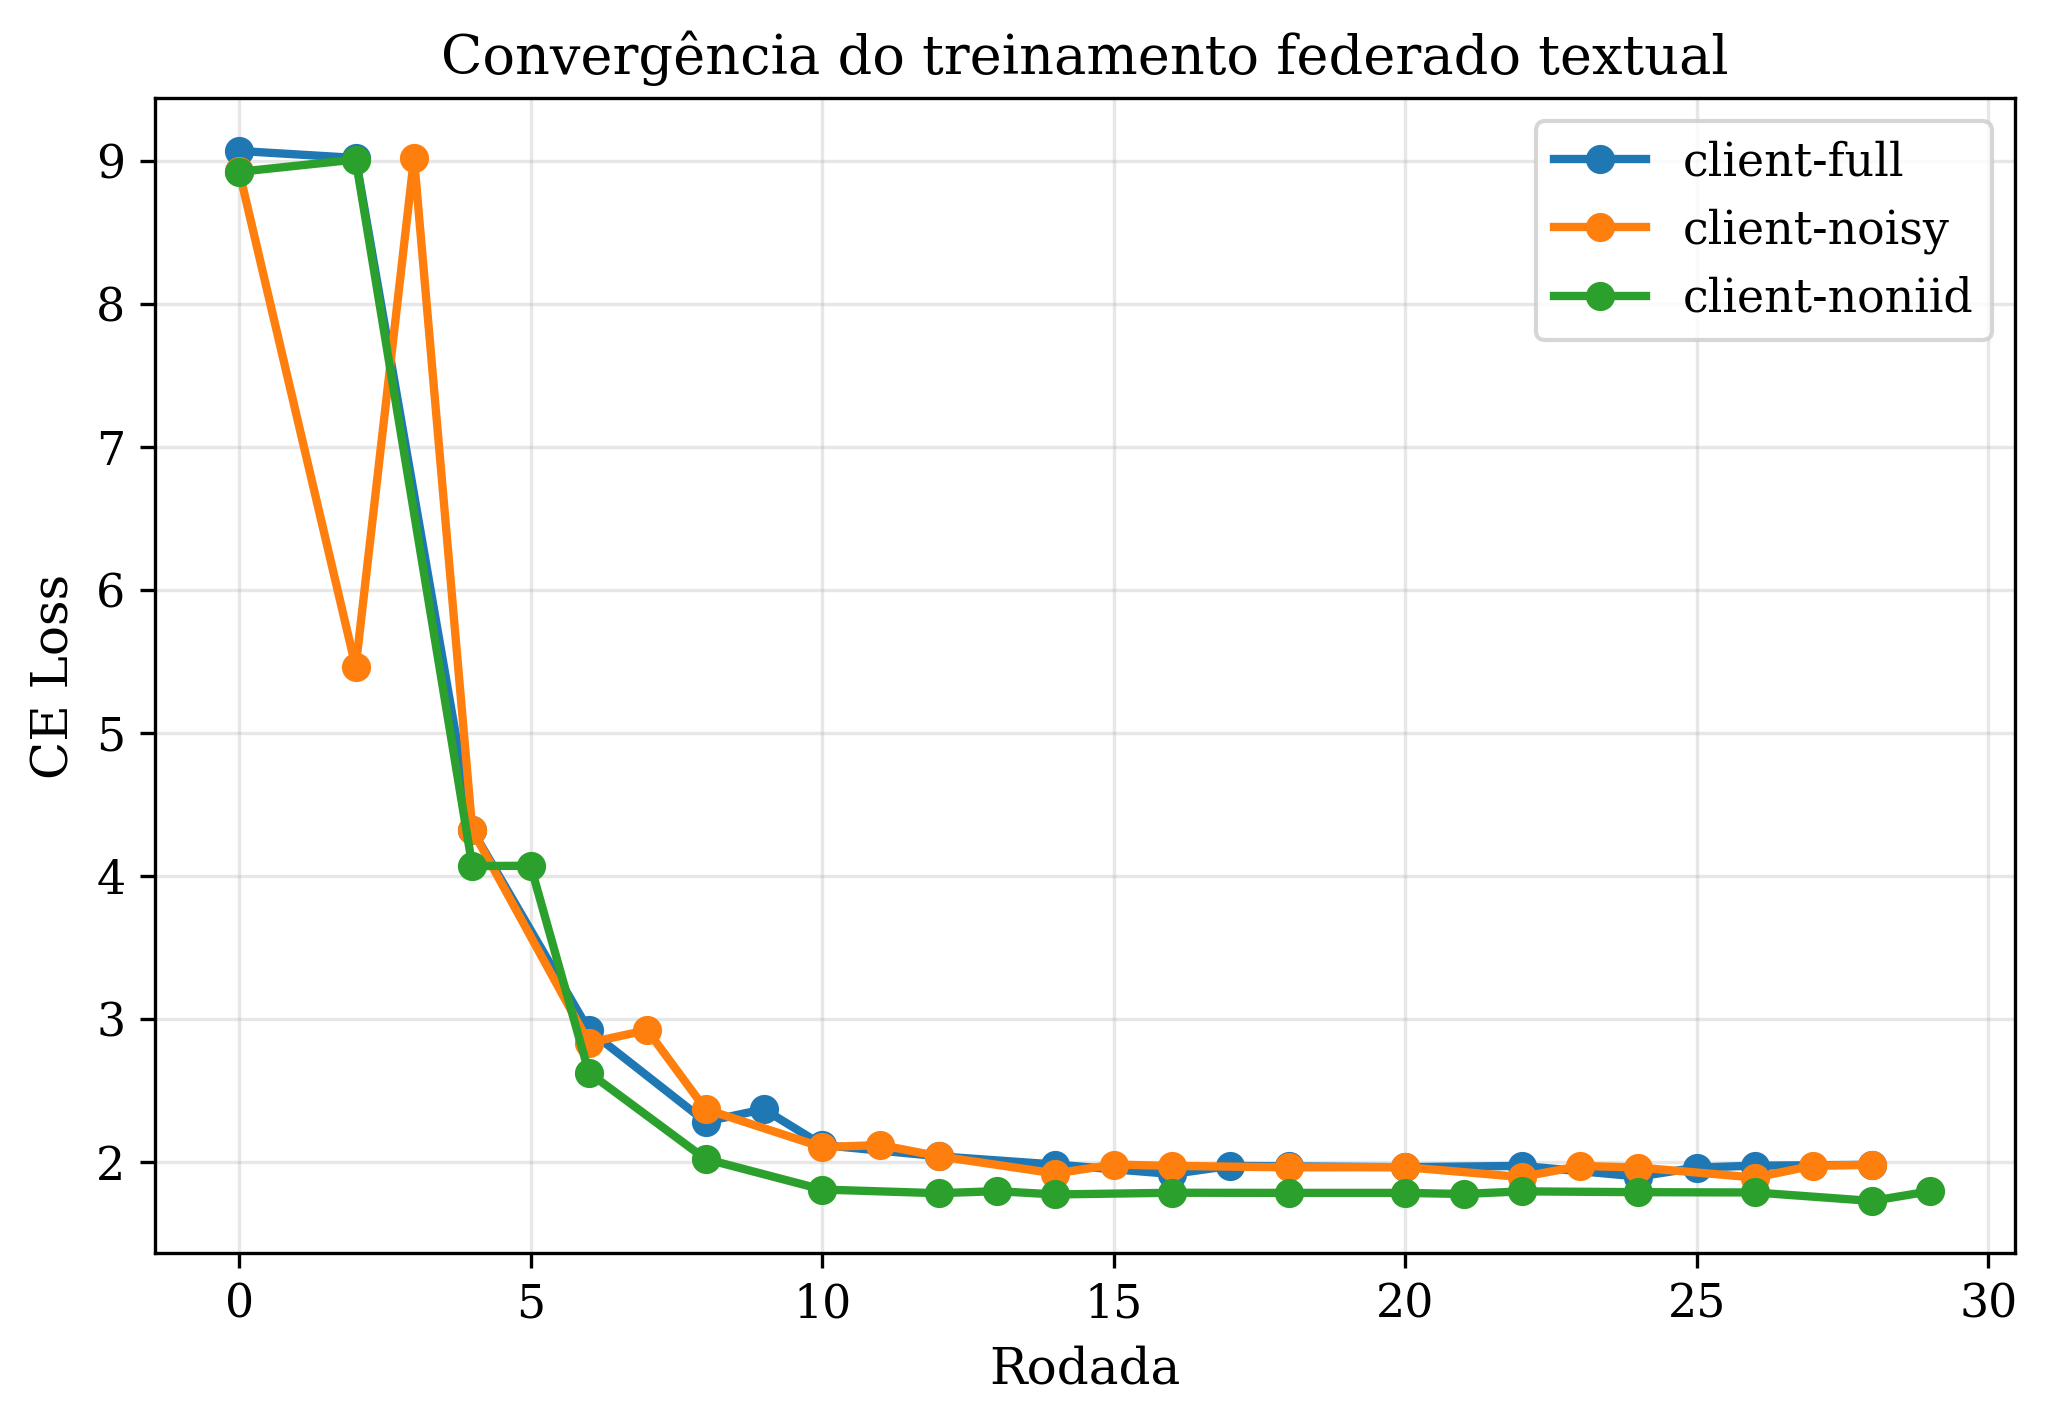
\includegraphics[width=\columnwidth]{figures/fig_convergence.png}
\caption{Convergência do treinamento federado textual no cenário base, com perda local agregada por rodada para cada cliente.}
\label{fig:convergence}
\end{figure}

O comportamento global por cenário está resumido na Tabela~\ref{tab:chaos_results} e ilustrado na Fig.~\ref{fig:chaos}. O melhor \ac{CE} observado foi 6,4480 no cenário \textit{Moderado}, enquanto a melhor acurácia global chegou a 35,0\% no cenário \textit{Normal}. O \ac{CE} final variou entre 6,8222 e 8,4104, e a acurácia final permaneceu concentrada entre 33,0\% e 34,0\%. Essa faixa estreita sugere que, com clientes quase homogêneos e corpus reduzido, a qualidade final do modelo depende mais da limitação do dataset e da capacidade do autoencoder do que da severidade do canal.

\begingroup\footnotesize
% Tabela gerada automaticamente por generate_figures.py
% Execute: python generate_figures.py para atualizar com dados reais
\begin{table}[htbp]
\centering
\caption{Impacto dos cenários de caos nas métricas de convergência.}
\label{tab:chaos}
\begin{tabular}{ccccc}
\hline
\textbf{Cenário} & \textbf{MSE Final} & \textbf{PSNR Final (dB)} & \textbf{Rounds até Convergência} & \textbf{Degradação (\%)} \\
\hline
Normal & --- & --- & --- & --- \\
Leve & --- & --- & --- & --- \\
Moderado & --- & --- & --- & --- \\
Severo & --- & --- & --- & --- \\
\hline
\end{tabular}
\end{table}

\endgroup

Para destacar a aproximação entre as condições dos clientes, a Tabela~\ref{tab:clients} resume os valores finais observados no cenário base. A diferença mais visível está no volume transmitido pelo cliente ruidoso, que caiu para aproximadamente 56~MB devido ao Top-K moderado, enquanto os demais permaneceram próximos de 66~MB. Em termos de perda local final, porém, os três clientes ficaram na mesma ordem de grandeza, reforçando que o objetivo desta configuração foi induzir diferenças leves, e não estabelecer um cliente excessivamente penalizado.

\begin{table}[t]
\centering
\caption{Comparabilidade entre clientes no cenário \textit{Normal}.}
\label{tab:clients}
\begin{tabular}{lcc}
\hline
\textbf{Cliente} & \textbf{Loss final} & \textbf{Bytes enviados} \\
\hline
client-full & 1,9796 & 66,3 MB \\
client-noisy & 1,9796 & 56,0 MB \\
client-noniid & 1,7943 & 66,3 MB \\
\hline
\end{tabular}
\end{table}

\begin{figure}[t]
\centering
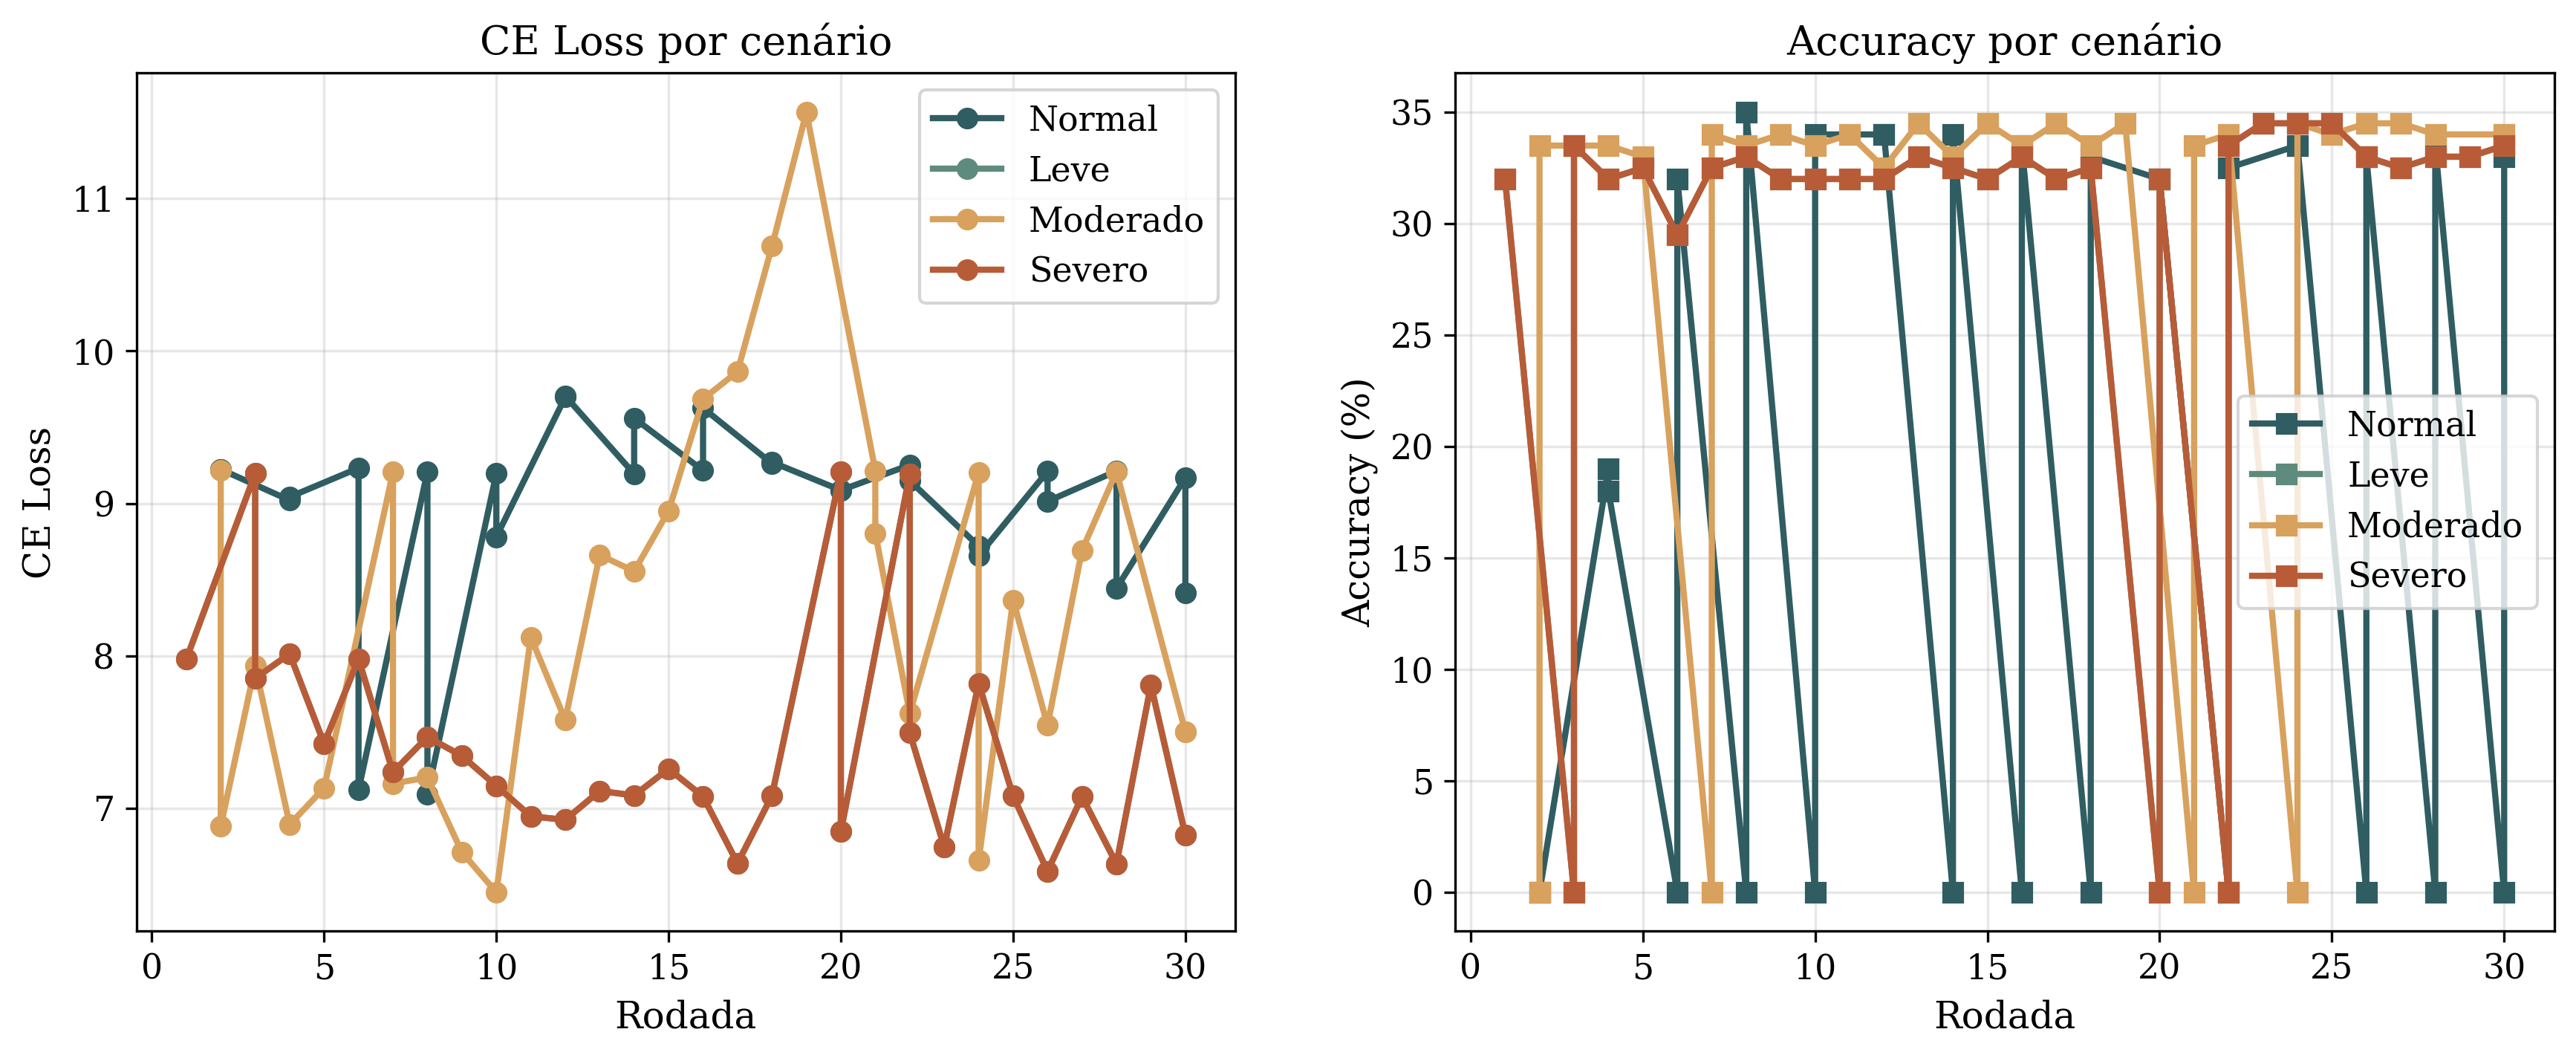
\includegraphics[width=\columnwidth]{figures/fig_chaos.png}
\caption{Comparação dos cenários de caos em termos de \ac{CE} global e acurácia global ao longo do treinamento.}
\label{fig:chaos}
\end{figure}

\subsection{Reconstrução Semântica}
A reconstrução textual por \textit{chunks} é mostrada na Fig.~\ref{fig:reconstruction}. O mecanismo de segmentação e remontagem funcionou adequadamente do ponto de vista estrutural: o sistema processou documentos com dois a três \textit{chunks}, retornou texto no destino e preservou o fluxo completo de inferência. Entretanto, a qualidade semântica ainda é modesta. A Tabela~\ref{tab:reconstruction} mostra \ac{CE} entre 15,2248 e 21,6409 e acurácia de tokens entre 0,0\% e 11,3\% nos exemplos amostrados.

Esse resultado é coerente com o restante do experimento: a infraestrutura está pronta e testada, mas o corpus é pequeno e a quantidade de rodadas ainda é insuficiente para reconstrução de alta fidelidade. Em outras palavras, o projeto já demonstra comunicação semântica textual funcional, porém a qualidade do conteúdo reconstruído ainda deve evoluir com corpus mais amplo, maior capacidade de modelo e mais iterações de treino.

\begin{figure*}[t]
\centering
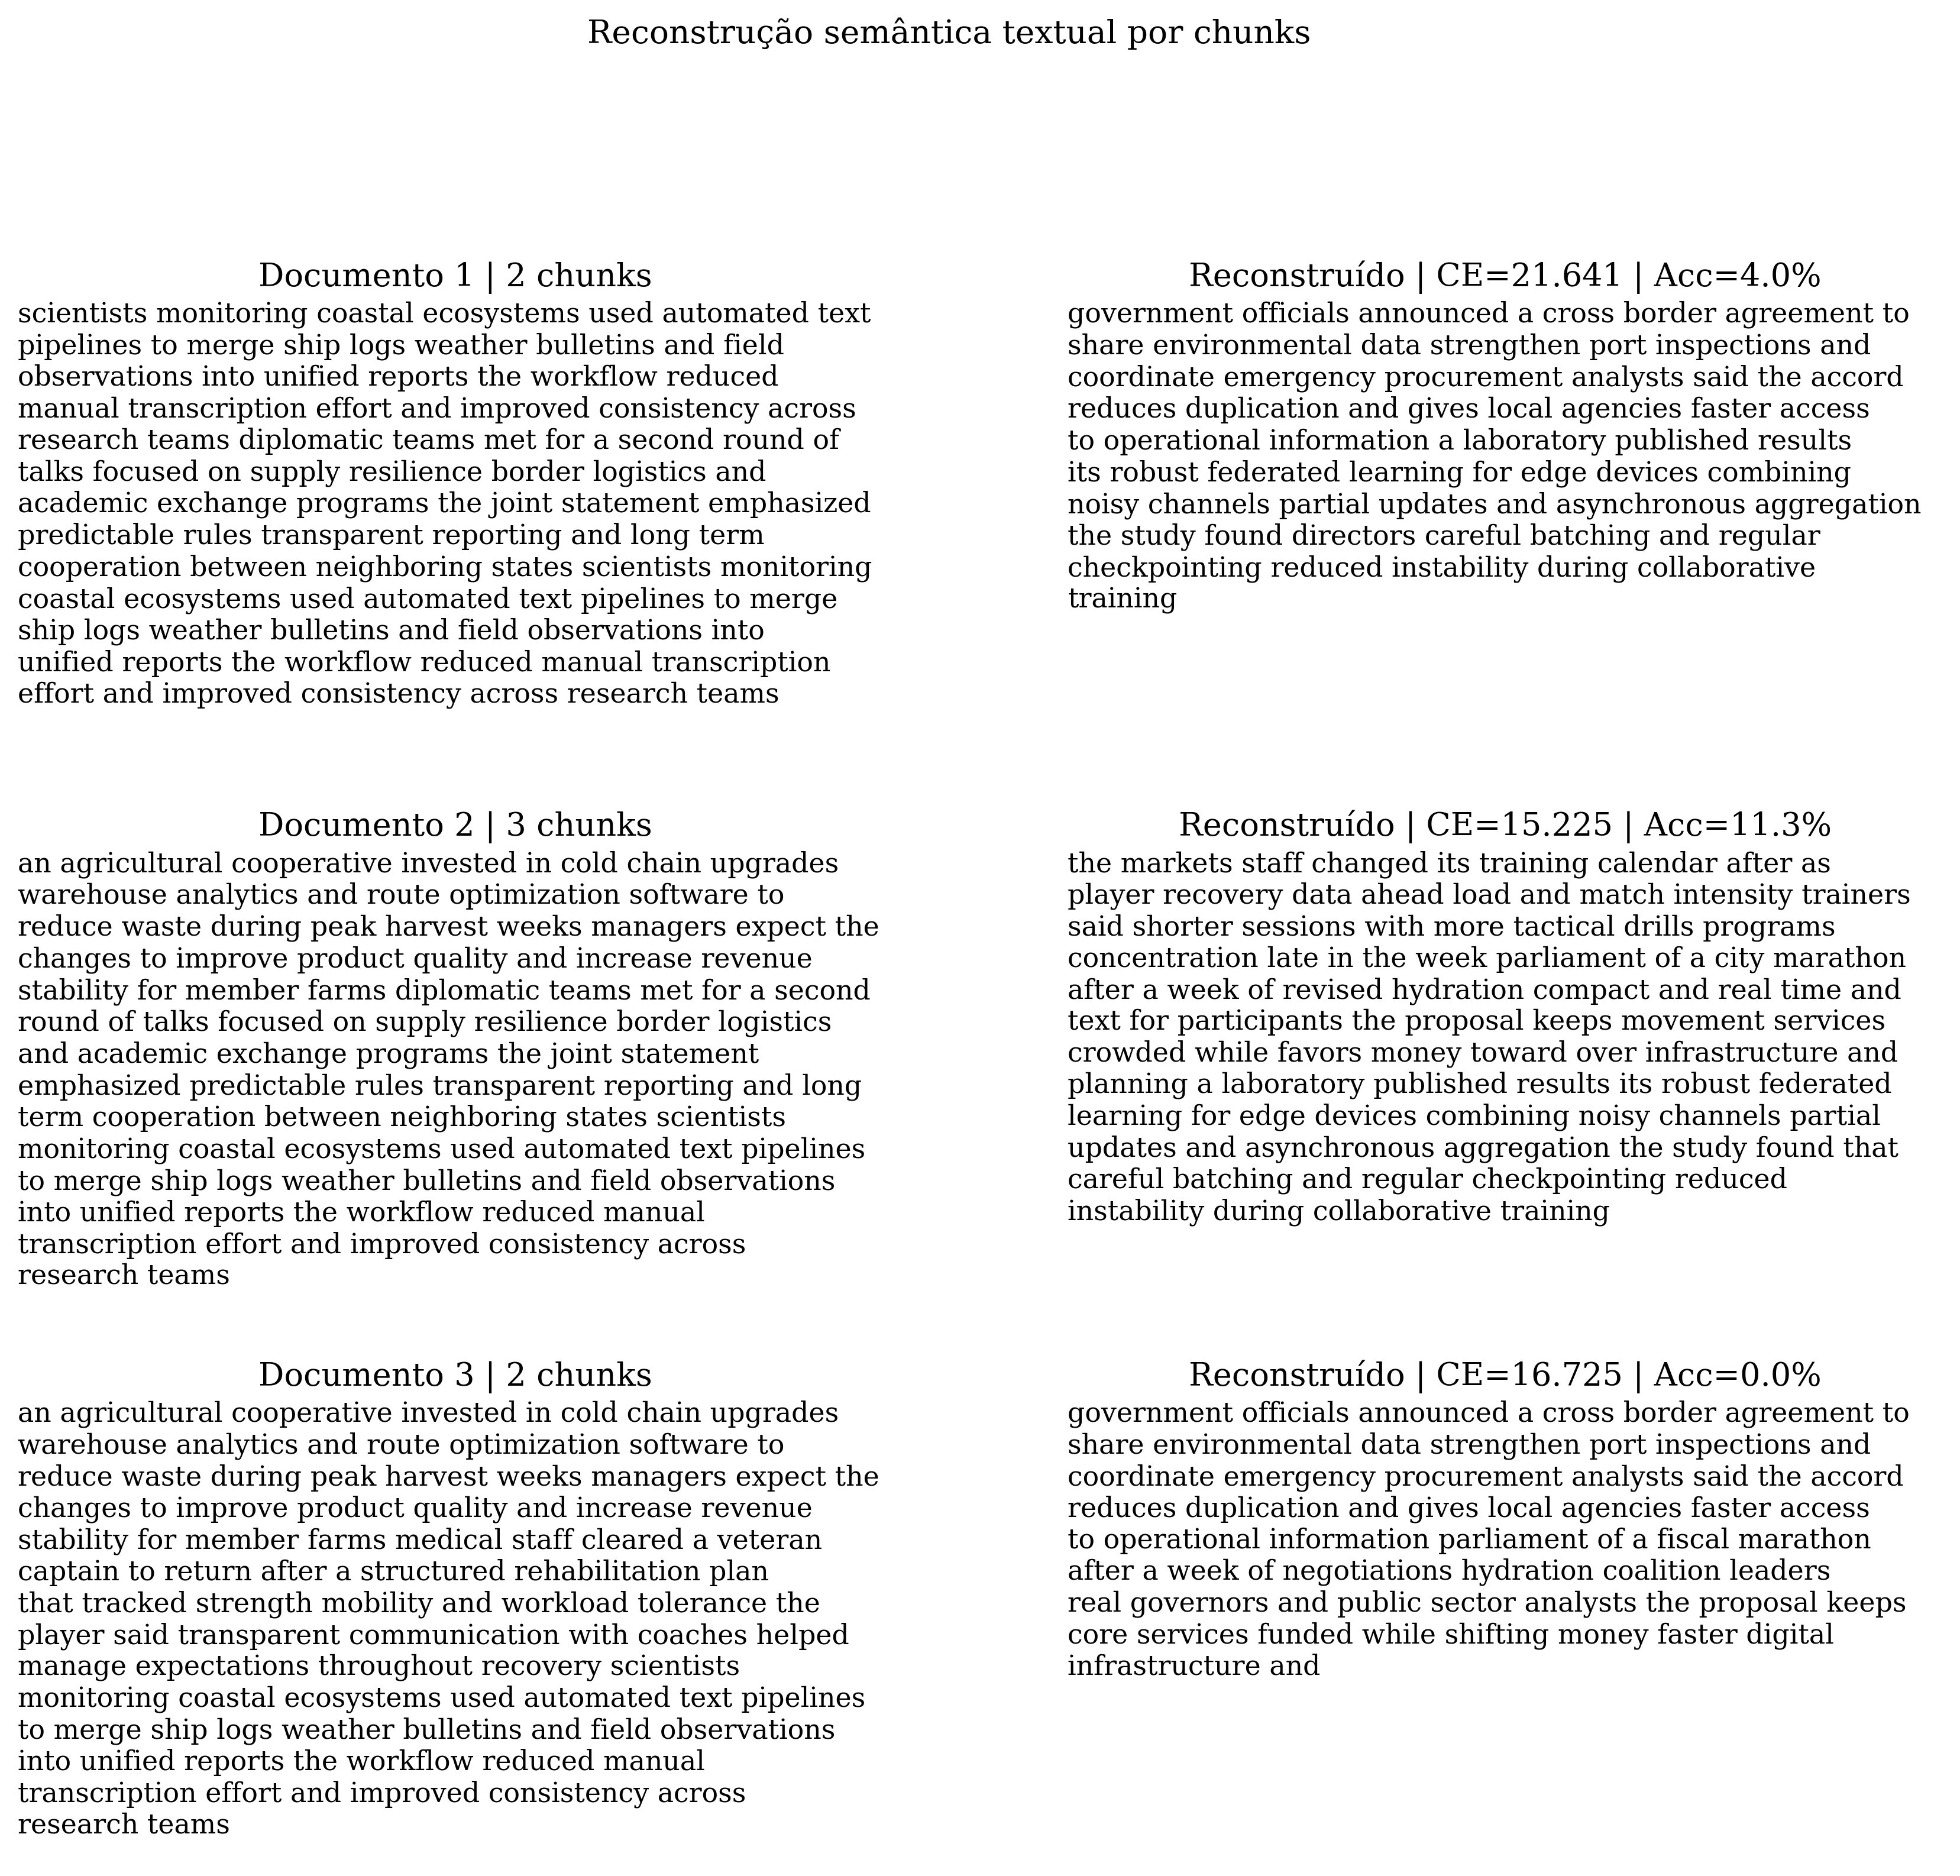
\includegraphics[width=0.97\textwidth]{figures/fig_reconstruction.png}
\caption{Exemplos qualitativos de reconstrução semântica textual por \textit{chunks}, com \ac{CE} e acurácia calculadas para cada documento.}
\label{fig:reconstruction}
\end{figure*}

\begingroup\footnotesize
\begin{table}[htbp]
\centering
\caption{Reconstrução semântica textual por documento.}
\label{tab:reconstruction}
\begin{tabular}{cccc}
\hline
\textbf{Documento} & \textbf{Chunks} & \textbf{CE Loss} & \textbf{Accuracy (\%)} \\
\hline
1 & 3 & 7.6272 & 12.0 \\
2 & 3 & 7.5126 & 12.0 \\
3 & 2 & 8.6736 & 4.0 \\
\hline
\end{tabular}
\end{table}

\endgroup

\subsection{Completação Textual}
A tarefa de completação, apresentada na Fig.~\ref{fig:completion}, foi avaliada com máscaras por truncamento e mascaramento aleatório. A Tabela~\ref{tab:completion} mostra que a estratégia aleatória de 40\% de máscara obteve \ac{CE} 41,7748, valor melhor do que os casos de truncamento, que atingiram 86,0969 e 111,4451. Em todos os casos, a acurácia permaneceu em 0,0\%, o que confirma que o sistema ainda não consegue completar trechos ausentes com precisão token a token.

Mesmo com esse resultado fraco em termos de qualidade, o experimento é útil por duas razões. Primeiro, ele comprova que o endpoint \texttt{/complete\_text} opera corretamente dentro da mesma arquitetura federada e containerizada usada no restante do projeto. Segundo, ele evidencia com clareza onde está a principal limitação do sistema: a infraestrutura já entrega o fluxo operacional, mas o modelo ainda precisa de mais capacidade de generalização semântica.

\begin{figure*}[t]
\centering
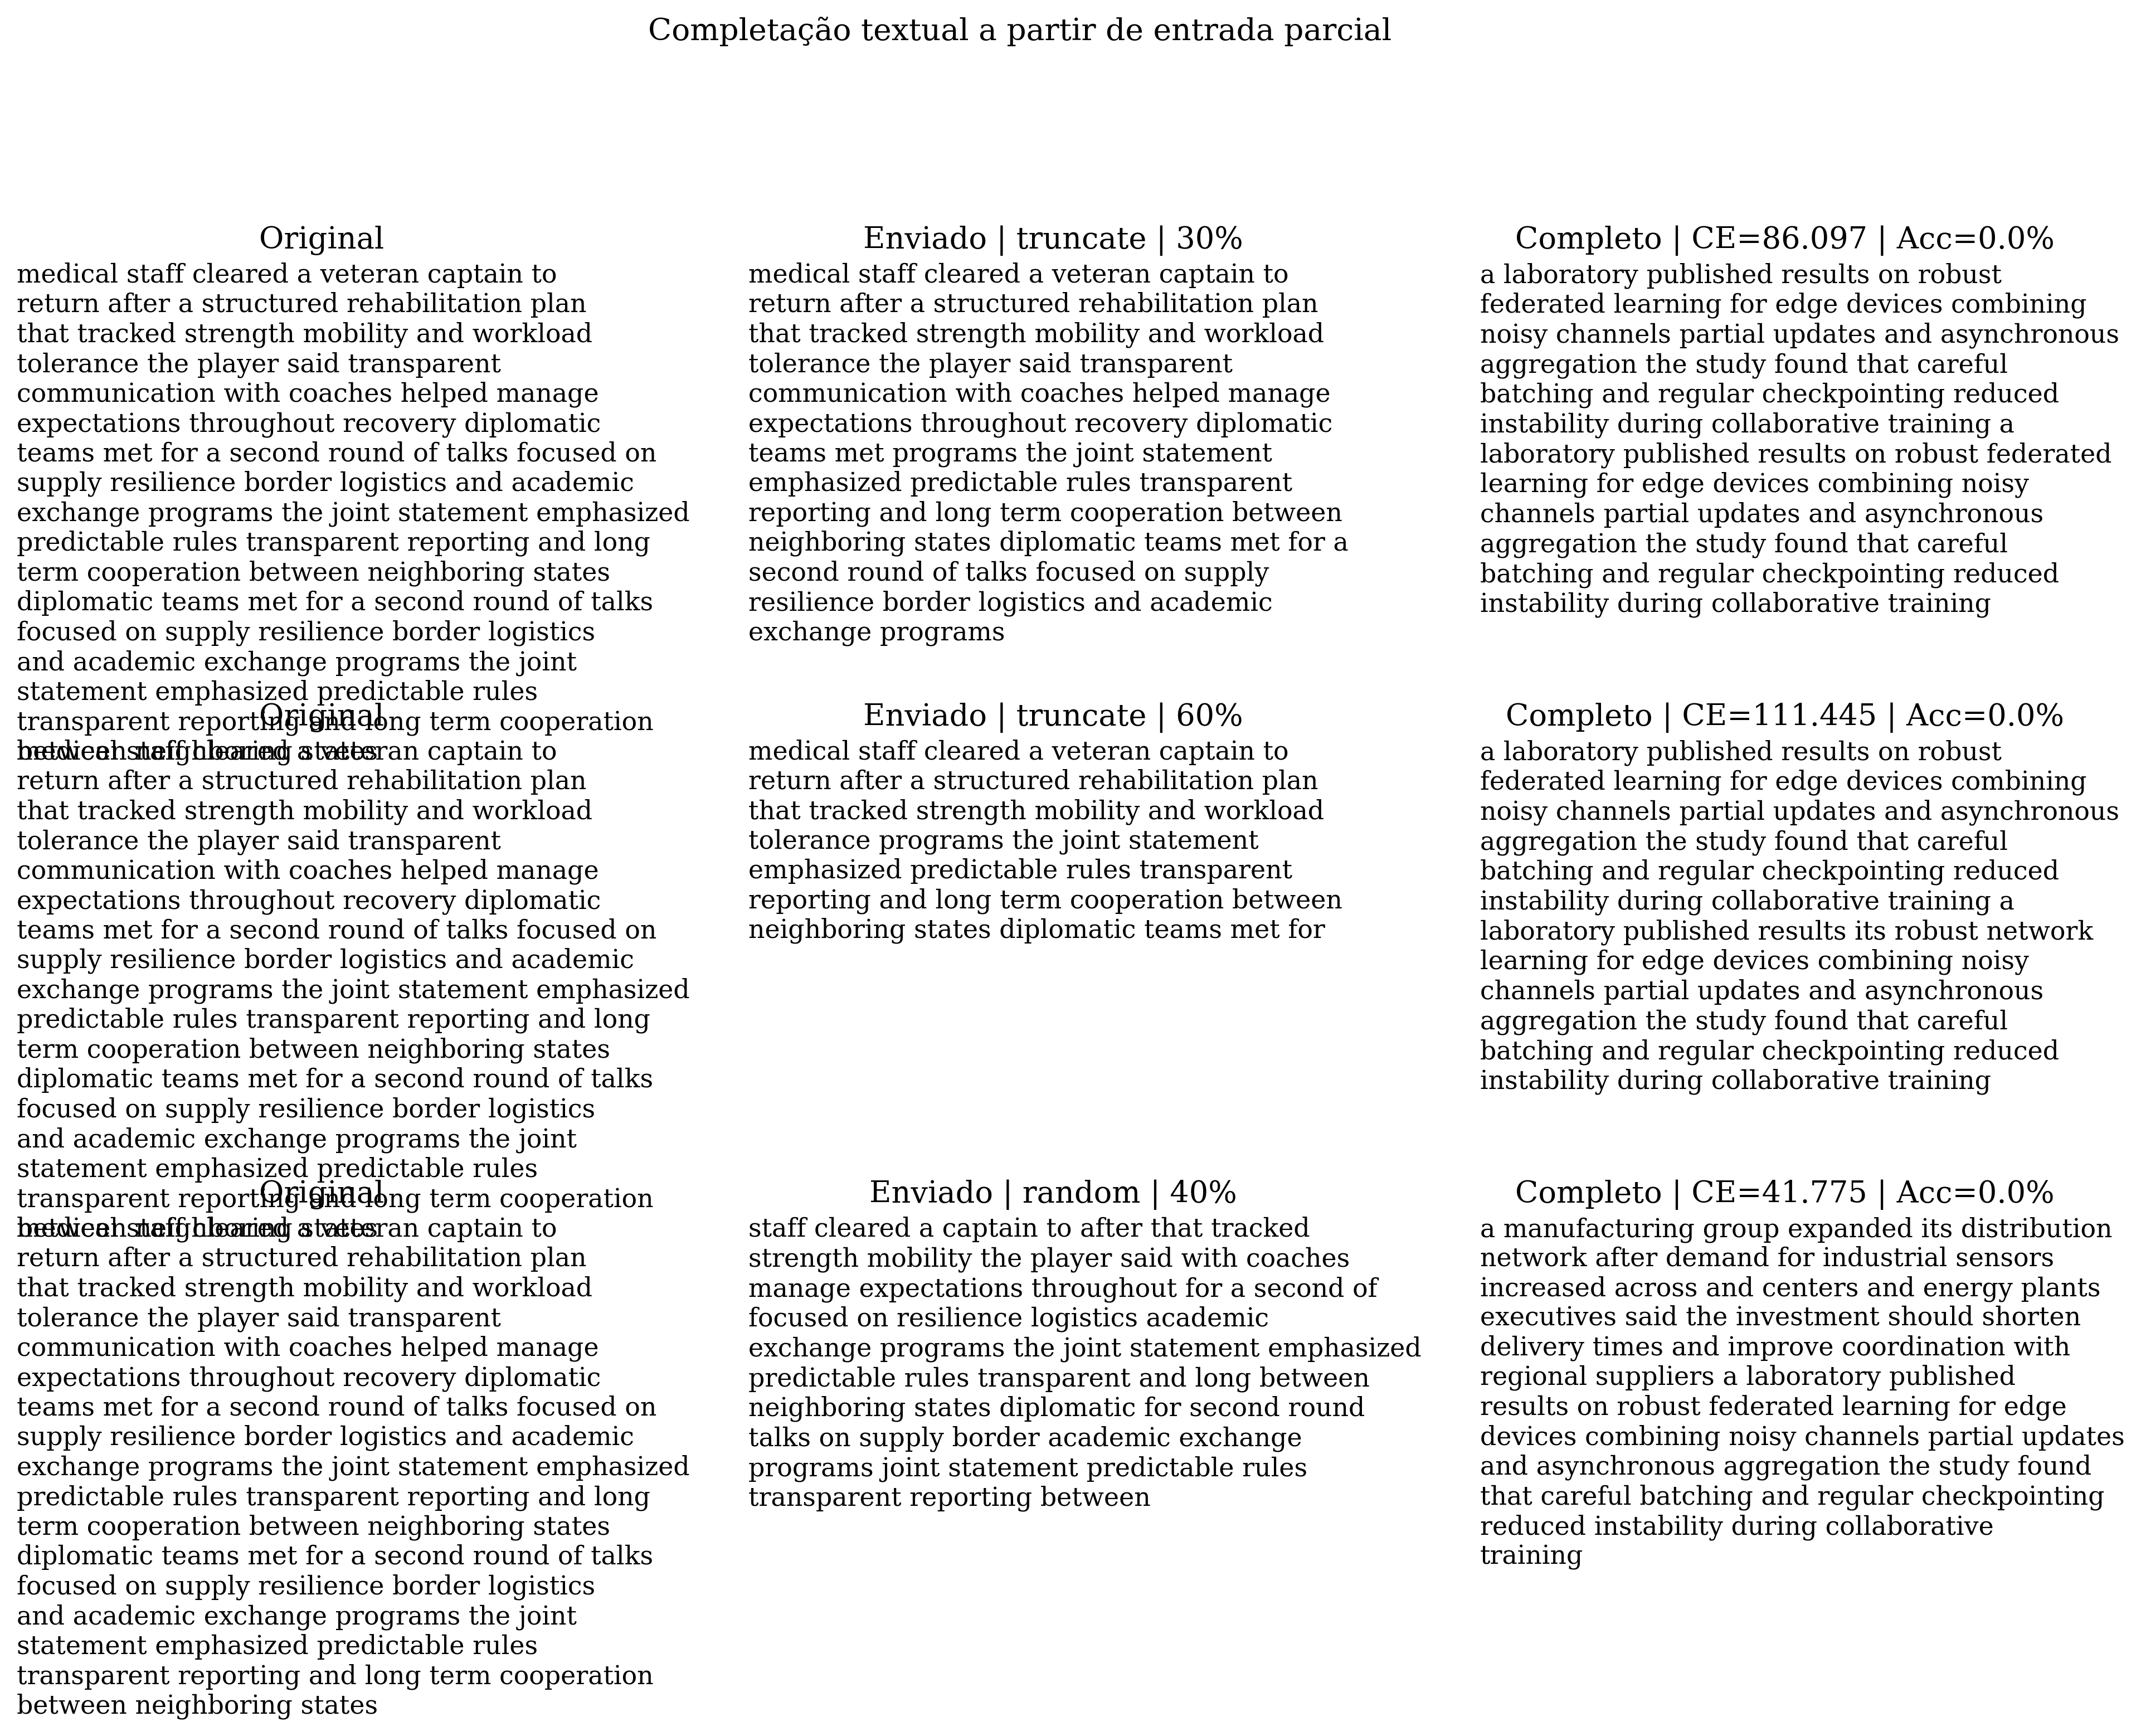
\includegraphics[width=0.97\textwidth]{figures/fig_completion.png}
\caption{Exemplos qualitativos da tarefa de completação textual a partir de entrada parcial, incluindo máscara enviada e saída completada.}
\label{fig:completion}
\end{figure*}

\begingroup\footnotesize
\begin{table}[htbp]
\centering
\caption{Completação textual por estratégia de mascaramento.}
\label{tab:completion}
\begin{tabular}{cccc}
\hline
\textbf{Estratégia} & \textbf{Máscara (\%)} & \textbf{CE Loss} & \textbf{Accuracy (\%)} \\
\hline
truncate & 30 & 86.0969 & 0.0 \\
truncate & 60 & 111.4451 & 0.0 \\
random & 40 & 41.7748 & 0.0 \\
\hline
\end{tabular}
\end{table}

\endgroup

No conjunto, os resultados indicam que a migração para um pipeline textual foi bem-sucedida do ponto de vista de engenharia. O sistema treina, agrega, exporta resultados, gera figuras, produz tabelas e atende chamadas de inferência entre contêineres. O ganho científico mais forte desta etapa não está em métricas absolutas altas, mas na consolidação de um ambiente reproduzível e coerente com comunicação semântica textual.

Também é importante notar que os resultados não seguem uma degradação monotônica com o aumento nominal da severidade do cenário. O cenário \textit{Moderado}, por exemplo, obteve o melhor \ac{CE} mínimo, enquanto \textit{Leve} e \textit{Severo} terminaram com valores finais idênticos nos CSVs exportados. Em vez de interpretar isso como um benefício direto do caos, a leitura mais prudente é que o regime atual ainda é dominado por ruído estatístico do corpus reduzido e pelo pequeno número de amostras de avaliação. Esse comportamento, longe de invalidar o experimento, deixa explícita a maturidade atual do sistema e aponta com clareza os próximos eixos de melhoria.

\subsection{Validação Operacional em Docker}
Além das métricas de treinamento, o software foi validado por execução autônoma em contêineres, incluindo subida do servidor, inicialização dos três clientes, aplicação do injetor de caos e chamadas reais aos endpoints \texttt{/compress\_text}, \texttt{/generate\_text} e \texttt{/complete\_text}. O fluxo retornou \textit{payloads} válidos, reconstruiu documentos por \textit{chunks} e produziu saídas textuais não vazias, confirmando que a arquitetura do projeto está funcional do ponto de vista de integração.

Esse resultado operacional é importante porque complementa a leitura das tabelas anteriores. Mesmo quando a qualidade da reconstrução ainda é baixa em nível de token, o sistema já atende ao objetivo desta fase: operar como um protótipo textual completo, capaz de treinar federadamente, transferir representações latentes e gerar artefatos de avaliação de forma reproduzível.

\section{Limitações e Ameaças à Validade}
Os resultados apresentados devem ser interpretados à luz de algumas limitações importantes. A primeira é o tamanho do corpus. O projeto usa, por escolha de engenharia, um conjunto textual embarcado e pequeno, suficiente para demonstrar o pipeline completo, mas insuficiente para treinar um codec semântico de alta qualidade. Isso afeta diretamente as tarefas de reconstrução e completação, nas quais a acurácia token a token permaneceu baixa.

A segunda limitação está nas próprias métricas. \ac{CE} e acurácia são úteis para acompanhar otimização e estabilidade, porém não capturam plenamente preservação semântica. Em comunicação semântica textual, uma reconstrução pode manter a ideia central sem reproduzir literalmente a sequência original. Portanto, parte da diferença entre a percepção qualitativa do sistema e os valores de acurácia decorre da escolha de métricas mais rígidas do que o objetivo final de significado.

Há também ameaças relacionadas ao desenho experimental. Embora quatro cenários tenham sido executados, o comportamento final não foi monotônico em relação à severidade nominal. Isso sugere que, no estágio atual, a variabilidade estatística do treino ainda é comparável ao efeito da perturbação de rede. Em outras palavras, o experimento mede corretamente a operação do sistema, mas ainda não isola com grande poder estatístico o impacto causal de cada cenário.

Outro ponto importante é a escala da federação. O estudo usa três clientes, o que é suficiente para validar agregação, heterogeneidade leve e compressão de pesos, mas ainda está distante de um ambiente federado amplo. Em cenários maiores, a combinação de atrasos, clientes intermitentes e distribuições mais heterogêneas tende a produzir efeitos mais fortes sobre convergência e qualidade final. Assim, os resultados deste artigo devem ser lidos como uma validação de plataforma e não como uma conclusão definitiva sobre o desempenho máximo da abordagem.

Mesmo com essas restrições, o valor do trabalho permanece claro. O sistema executado aqui fecha um ciclo completo: treinamento federado, exportação de resultados, validação de endpoints e compilação automática de artefatos para documentação científica. Isso cria uma base concreta para iterações posteriores, nas quais melhorias de corpus, arquitetura e métrica poderão ser avaliadas sobre uma infraestrutura já consolidada.

\section{Conclusão}
Este artigo apresentou a versão textual e containerizada de um framework de comunicação semântica baseado em \ac{FL}. O sistema foi executado de ponta a ponta com três clientes em condições quase homogêneas, geração automática de métricas e validação real dos endpoints de compressão, reconstrução e completação. Os experimentos mostraram estabilidade global entre os cenários testados, com \ac{CE} final entre 6,82 e 8,41 e acurácia global próxima de 34\%, ao mesmo tempo em que evidenciaram a limitação qualitativa do modelo atual na reconstrução e na completação de documentos.

Como trabalhos futuros, recomenda-se ampliar o corpus textual, aumentar a diversidade semântica, testar \ac{VAE} como modo padrão e explorar métricas adicionais mais próximas de similaridade semântica. Ainda assim, o objetivo central desta fase foi atingido: o projeto deixou de ser um protótipo híbrido e passou a operar como uma plataforma textual completa, reproduzível e pronta para iterações experimentais posteriores.

\bibliographystyle{IEEEtran}
\bibliography{ref}

\end{document}